\documentclass[oneside,12pt]{wipb}
\usetikzlibrary{mindmap,trees}

\usepackage[polish, english]{babel}
\usepackage{textcomp,mathcomp}
\usepackage{url}
\def\UrlBreaks{\do\/\do-}
\usepackage{breakurl}
\usepackage[breaklinks]{hyperref}

\typpracy{INŻYNIERSKA}
\temat{System monitorowania parametrów środowiska w pomieszczeniach z użyciem Raspberry Pi}
\autor{Kacper Bajeński}
\promotor{dr inż. Marcin Adamski}
\indeks{107598}
\studia{stacjonarne}
\rokakademicki{2022/2023}
\profil{stacjonarne I stopnia}
\kierunekstudiow{informatyka}
\specjalnosc{}
\zakres{1. Analiza wymagań I \newline 2. Przegląd i wybranie technologii \newline 3. Projekt i implementacja aplikacji}

\hypersetup{ %wpisy w pdf info
pdfauthor={mgr inż. Maciej Brzozowski},
pdftitle={Opis użycia klasy wipb},
pdfsubject={},
pdfkeywords={Praca dyplomowa},
pdfpagemode=UseNone,
linkcolor=black,
citecolor=black
} 

\begin{document}
\selectlanguage{polish}
\maketitle
\tableofcontents
\thispagestyle{empty}
\setcounter{page}{0}
\pagestyle{plain}

\chapter{Wstęp}

Problem pomiarów parametrów środowiska jest powszechny w każdej dziedzinie życia.
Wykonywanie ich pomaga nam w życiu codziennym przy prostych czynnościach jak
wybieranie ubioru odpowiedniego do pogody, ale również przydaje się w bardziej
zaawansowanych sferach jak badania naukowe. Częstym zastosowaniem są również
domowe hodowle roślin, które wymagają stałego monitorowania parametrów
takich jak temperatura czy wilgotność, aby zapewnić im odpowiednie warunki
do rozwoju. Innym przykładem użyteczności takiego rozwiązania są automatyczne
systemy kontroli jakości powietrza w pomieszczeniach. Mogą się one składać
z uzdatniaczy powietrza, klimatyzatorów, pieców, itp. Taki system monitorowania
może wydawać komendy tym urządzeniom w celu automatycznej i precyzyjnej kontroli
w czasie zbliżonym do rzeczywistego.

Celem pracy jest stworzenie systemu pozwalającego na odczyt parametrów środowiska
w pomieszczeniach oraz ich przechowywanie. Stworzone oprogramowanie powinno pozwalać
na zapis dowolnych danych z różnego rodzaju sensorów oraz ich późniejszy odczyt
przez użytkownika. Powinien również powstać system powiadomień informujący
użytkownika o niespodziewanych wartościach odczytów.
Część systemu zajmująca się monitorowaniem oraz przesyłem
parametrów została zrealizowana przy użyciu komputera Raspberry Pi, a
interfejs użytkownika przyjął formę strony internetowej. Całość komunikuje się
z centralnym serwerem, który przechowuje oraz udostępnia dostęp do
zapisanych na nim danych.

W następnych rozdziałach zostały opisane następujące zagadnienia:
\begin{itemize}
  \item szczegółowa analiza problemu monitorowania parametrów środowiska.
    Opisano tam zastosowania takiego systemu oraz wymagania jakie powinien
    on spełniać.
  \item podobne rozwiązania wraz z ich wadami oraz zaletami,
  \item wybrane technologie do implementacji systemu,
  \item szczegóły implementacji systemu,
  \item podsumowanie wraz z oceną zaimplementowanego rozwiązania.
\end{itemize}

\chapter{Analiza problemu}

Problem pomiarów parametrów środowiska jest powszechny w każdej dziedzinie życia.
Wykonywanie ich pomaga nam w życiu codziennym przy prostych czynnościach jak
wybieranie ubioru odpowiedniego do pogody, ale również przydaje się w bardziej
zaawansowanych sferach jak badania naukowe. Częstym zastosowaniem są również
domowe hodowle roślin, które wymagają stałego monitorowania parametrów
takich jak temperatura czy wilgotność, aby zapewnić im odpowiednie warunki
do rozwoju. Innym przykładem użyteczności takiego rozwiązania są automatyczne
systemy kontroli jakości powietrza w pomieszczeniach. Mogą się one składać
z uzdatniaczy powietrza, klimatyzatorów, pieców, itp. Taki system monitorowania
może wydawać komendy tym urządzeniom w celu automatycznej i precyzyjnej kontroli.

Zwracając uwagę na powszechność problemu oraz ilość możliwych parametrów,
które można zmierzyć, stworzony system powinien umożliwiać na obsługę jak 
największej grupy rodzajów odczytów. Zależnie od przeznaczenia użytkownik
powinien mieć możliwość wykorzystania jak największej grupy sensorów ze
zdolnością do wykonywania odczytów różnych parametrów środowiska.
Taka implementacja możliwa jest poprzez stworzenie generycznego rozwiązania, które
nie ograniczałoby użytkownika i na jego podstawie tworzenie oprogramowania
sterującego danym modelem urządzenia.
Może być to osiągnięte z użyciem odpowiednich poziomów abstrakcji w oprogramowaniu.
Umożliwiłoby to również na zwiększoną modularność rozwiązania oraz
wyłączenie niewymaganych w danym zastosowaniu składników systemu.
Dzięki temu zmniejszona zostaje złożoność oraz rozmiar oprogramowania
na urządzeniu monitorującym.

Niektóre sytuacje mogą wymagać reakcji człowieka na zdarzenie, np.
w przypadku niespodziewanego uszkodzenia, którejś z części kontrolującej
temperaturę powietrza. W takich przypadkach dobrym rozwiązaniem jest możliwość
wysyłania powiadomień użytkownikowi o niestandardowym zachowaniu.
Mogą być to informacje o przekroczeniu skonfigurowanej wartości danego czynnika
lub niespodziewanej nagłej jego zmianie. Taki system notyfikacji wraz z
częstym odczytem parametrów może znacznie przyśpieszyć czas reakcji
i naprawy problemu, co może przełożyć się na znacznie zredukowane straty.
Taki system mógłby zostać również wykorzystany do notyfikowania innych
urządzeń o zmianach parametrów tym samym pozwalając na automatyzację
ich działania oraz konfiguracji. Urządzenie mogłoby reagować na daną 
informację i sama dostosować swoje działanie lub w bardziej zaawansowanych
przypadkach logika biznesowa mogłaby znaleźć się po stronie serwera i 
kontrolować pracę tego urządzenia.

Do wielu zastosowań może być również konieczne przeglądanie odczytów historycznych.
Taka funkcjonalność jest konieczna w przypadku, np. badań wpływu danych
parametrów środowiska na badany obiekt. Umożliwia to na ułatwioną korelację
wartości odczytów ze zmianami w podmiocie badań. Przydaje się również 
wraz z wykorzystaniem systemów poprawiających jakość czy temperaturę
powietrza, gdzie porównując wykorzystaną moc urządzenia możemy skorelować
ze zmianami parametrów środowiska wraz z biegiem czasu.
Aplikacja powinna więc mieć możliwość zapisu oraz odczytu danych. Powinny być
one przechowywane w formacie, który umożliwi późniejsze ich łatwe przetwarzanie,
co pomoże w przypadku budowy innych funkcjonalności na zgromadzonych danych
jak również ułatwi samą ich prezentację użytkownikowi. Funkcjonalnością, która
powinna się również pojawić powinna być możliwość filtrowania oraz sortowania
odczytów przez użytkownika.


\chapter{Analiza istniejących rozwiązań}
Ze względu na powszechność problemu przedstawionego w tej pracy na przestrzeni lat powstało wiele 
systemów umożliwiających rozwiązanie go w mniejszym lub większym stopniu. 
Ich eksploracja może ułatwić wytworzenie podobnego systemu poprzez zauważenie mocnych i słabych
stron danego rozwiązania. Na ich podstawie możliwa jest adopcja oraz usprawnienie danych składowych
systemu w przypadku zalet oraz poprawa lub zastąpienie innym rozwiązaniem w przypadku wad.


W tym rozdziale zostaną poddane analizie niektóre z tych systemów w celu określenia ich 
wad i zalet oraz wyszczególnienia brakującej, bądź też niepełnej funkcjonalności.

\section{Kryteria analizy porównawczej}
Analiza porównawcza odbędzie się na podstawie następujących kryteriów:
\begin{itemize}
  \item typ parametrów, które dany system pozwala obserwować;
  \item zakres pomiarów;
  \item częstotliwość pomiarów;
  \item sposób komunikacji;
  \item sposób przechowywania danych;
  \item koszt wdrożenia;
  \item możliwość rozbudowy.
\end{itemize}
Zastosowanie tych parametrów powinno umożliwić szczegółowy przegląd dostępnych aktualnie
rozwiązań oraz wskazanie punktów, które mogą zostać w znaczny sposób usprawnione.

\section{System Verkada SV11}
Verkada SV11 jest wielofunkcyjnym urządzeniem \cite{verkada:sv11} pozwalającym na odczyt wielu
parametrów środowiska. System ten jest w stanie odczytać poniższe wartości:
\begin{itemize}
  \item temperaturę pomieszczenia w zakresie $-5 - 50 ^\circ C$,
  \item wilgotność powietrza w zakresie $0-80\%$,
  \item aerozole atmosferyczne o średnicy mniejszej niż $2,5\mu m$ (PM2,5) w zakresie $0-1000\mu g/m^3$,
  \item poziom głośności w zakresie $20 - 120dB$,
  \item wskaźnik jakości powietrza (ang. \emph{Air Quality Index}) zgodnie ze standardem USEPA (ang. \emph{United States Environmental Protection Agency}),
  \item ruch za pomocą detektora podczerwieni.
\end{itemize}
Pomiary wykonywane są w czasie zbliżonym do czasu rzeczywistego wykorzystując sieć Internet
poprzez połączenie typu Ethernet z zasilaniem w technologii PoE (ang \emph{Power over Ethernet}). 
Technologia wykorzystywana w sensorach firmy Verkada wymaga stałego połączenia z chmurą, 
dzięki czemu użytkownik nie musi dbać o przechowywanie czy przetwarzanie danych, ale
wiąże się to z dodatkowymi opłatami abonamentowymi i limitowaną funkcjonalnością w zależności
od poziomu subskrypcji. System pozwala na przeglądanie danych aktualnych oraz historycznych, a
przy dodatkowej opłacie udostępnia tryb alertów pozwalający na notyfikowanie użytkowników o
niespodziewanych zdarzeniach, takich jak przekroczenie wartości danych parametrów.
Koszt systemu jest najwyższy z przedstawionych w tej analizie i dodatkowo bazuje on na
modelu subskrypcyjnym co sprawia, że może być on poza zasięgiem dla większości osób i jest
głównie przeznaczony dla dużych firm.
Pod warunkiem wykorzystania jedynie urządzeń tej firmy system może być rozbudowany o 
dodatkowe sensory, kamery, alarmy czy też urządzenia kontroli dostępu. Urządzenia oraz
oprogramowanie innych producentów nie może z nimi współpracować.

\section{System SensorPush}
System SensorPush umożliwia na monitorowanie podstawowych parametrów takich jak temperatura,
wilgotność i ciśnienie powietrza. Produkt jest w stanie odczytywać z dużą dokładnością pomiary temperatury
w zakresie $0 - 60 ^\circ C$, wilgotność powietrza w zakresie $0-80\%$ i ciśnienie powietrza w zakresie 
$300 - 1250mb$. Urządzenie pracuje całkowicie używając zasilanie bateriami CR2477 co zwiększa
jego przenośność, gdyż nie potrzebne jest zewnętrzne źródło energii elektrycznej. 
W wersji bez dodatkowej bramy WiFi produkt wykorzystuje połączenie z użyciem technologii
Bluetooth w celu przesyłania odczytów do aplikacji sterującej. 
Najmniejszy możliwy interwał odczytów wynosi 1 minutę.
System pozwala na połączenie wielu sensorów tego producenta z jego
oprogramowaniem i monitorowanie aktualnych oraz historycznych odczytów. Główną limitacją
jest połączenie Bluetooth i jego zasięg przez co nie zawsze jest możliwe uzyskanie dobrego
zasięgu obsługi. Producent oferuje dodatkową bramę WiFi, z którą możliwe jest sparowanie
sensorów oraz następnie przesyłanie przez nią danych i zapis w chmurze. Ta usługa płatna
jest tylko przy zakupie urządzenia następnie producent zapewnia do niej dostęp bez dodatkowych opłat.
Dzięki temu rozwiązaniu możliwy jest dostęp do danych wszędzie z dostępem do sieci Internet.
Dodatkowo aplikacja wyposażona jest w system alertów, które użytkownik może otrzymywać przy odpowiedniej
konfiguracji, np. przy przekroczeniu danej wartości temperatury. Te notyfikacje prezentowane są
jako powiadomienia wykorzystując urządzenie, na którym zainstalowana jest aplikacja.

\section{System TempStick}
TempStick jest prostym urządzeniem pozwalającym na monitorowanie temperatury oraz wilgotności powietrza.
Urządzenie pozwala na odczyt temperatury w zakresie $5 - 60 ^\circ C$ i wilgotności w zakresie $0-100\%$.
Zasilany jest z użyciem baterii AA i nie wymaga dodatkowego źródła energii.
Przesyłanie danych odbywa się z użyciem sieci WiFi po wcześniejszym sparowaniu urządzenia z aplikacją
producenta. Odczyty z sensorów przesyłane są bezpośrednio do serwisu chmurowego, skąd mogą być następnie
pobrane w celu sprawdzenia aktualnych i historycznych wartości. Producent zapewnia do nich dostęp bez
dodatkowych opłat. System pozwala na połączenie wielu sensorów tego wytwórcy do jednego konta
użytkownika co umożliwia jednoczesny odczyt ich danych. Minimalny interwał czasu pojedynczego
odczytu wynosi 5 minut. System umożliwia również konfigurację notyfikacji przy przekroczonych 
wartościach oraz alertów o utraconym połączeniu czy wyczerpującej się baterii. Zakładając istnienie 
wcześniejsze infrastruktury WiFi koszt wprowadzenia jest niski.

\section{Podsumowanie}
Przedstawione urządzenia cechują się podobnym zakresem możliwych pomiarów. Można z tego wnioskować, że
większość sensorów dostępnych aktualnie na rynku będzie zachowywać się podobnie. Nie jest więc to
zagadnienie, które można w łatwy sposób usprawnić.


Zupełnie inaczej jest w przypadku typu pomiarów jakie możemy wykonywać. Podstawowymi parametrami są
temperatura i wilgotność powietrza, które można odczytać za pomocą większości rozwiązań tego typu.
Systemy z możliwością uchwycenia dodatkowych czynników środowiska zazwyczaj są znacznie droższe, a
urządzenia nie mogą być w przyszłości rozbudowane o dodatkowe sensory. Jest to punkt, który jest możliwy
do poprawy z użyciem systemu Raspberry Pi i wytworzeniu adekwatnie uniwersalnego oprogramowania, które umożliwiałoby
użytkownikowi na definiowanie własnych parametrów oraz dodawanie nowych sensorów.


Częstotliwość pomiarów również jest punktem, który mógłby ulec polepszeniu. Oprócz najdroższej opcji
przedstawionej w tej pracy żadna z nich nie jest w stanie działać w czasie zbliżonym do rzeczywistego
i pomiary wykonywane są w odstępach liczonych w minutach. Może być to niewystarczające w wielu przypadkach
użycia takiego systemu, a z użyciem odpowiedniej platformy interwał na poziomie kilku sekund nie powinien być
trudny do osiągnięcia.


Każda z przedstawionych solucji wykorzystuje różne sposoby połączenia urządzeń z siecią. Ze wszystkich
najlepszym wydaje się być ten z systemu SensorPush. W dzisiejszych czasach sieci WiFi są bardzo powszechne
i nie powinno to w większości przypadków generować dodatkowych kosztów. W porównaniu z wykorzystaniem 
technologii Bluetooth sieci bezprzewodowe WiFi cechują się znacznie większą niezawodnością oraz
większym zasięgiem działania. Natomiast sieć Ethernet mimo, że jest najbardziej niezawodna z nich
niesie za sobą dodatkowe problemy logistyczne takie jak rozłożenie kabli w budynkach, co w niektórych
przypadkach jak, np. obiekty zabytkowe może być niemożliwe.


Wszystkie przedstawione systemy wykorzystują technologie chmurowe do przechowywania danych.
Niesie to ze sobą wiele korzyści takich jak ułatwiony dostęp w każdym miejscu z połączeniem z
siecią Internet, ale niesie też ze sobą w niektórych przypadkach dodatkowe koszty.
Innym problemem jest przypadek braku dostępu do danego serwisu lub całkowite wygaśnięcie oferowanej
usługi. W takim przypadku dane urządzenia stają się bezużyteczne, a cały system należy migrować
do rozwiązań innego producenta. Problem ten można prosto rozwiązać oddając kontrolę nad
serwerem klientowi. Oczywiście wymaga to, aby proces wdrażania systemu był jak najprostszy, żeby
mógł trafić on do jak największej liczby osób.


Żaden z przedstawionych systemów nie pozwala na prawdziwą rozbudowę poza tym co oferuje 
dany producent. Sensory różnych producentów nie mogą być połączone z systemem innych.
Może zostać to rozwiązane poprzez publikację standardu, który taka aplikacja obsługuje.
Pozwoliłoby to na implementację różnych rozwiązań bazujących na dowolnej platformie.


\chapter{Wybrane technologie}

W tym rozdziale opisane zostaną technologie użyte do rozwiązania zadanego problemu.
System został podzielony na różne komunikujące się ze sobą aplikacje i każda z nich
wymaga różnego podejścia do ich wytworzenia. Z tego powodu ten rozdział został podzielony
na podrozdziały, każdy z nich opisujący dany program i technologie użyte do ich
utworzenia.

\section{Aplikacja kliencka}
Aplikacja kliencka została wykonana w formie strony internetowej.

\subsection*{WebAssembly}
WebAssembly to technologia opisująca standardowy kod binarny oraz jego reprezentację tekstową,
niezależne od platformy jego wykonania \cite{mdn:wasm, wasm:standard}. Umożliwia to
tworzenie przenośnego oprogramowania, które może zostać wykorzystane w wielu różnych systemach.
Głównymi celem WebAssembly jest umożliwienie tworzenia szybkiego oraz bezpiecznego pod względem
obsługi pamięci oprogramowania, które może być stworzone w dowolnym języku programowania, 
niezależnie od platformy oraz sprzętu, na którym ma być wykonywane \cite{wasm:standard}.

\subsection*{Rust}
Rust to wielo-paradygmatowy kompilowany język programowania. Oznacza to, że łączy ze sobą cechy różnych
konwencje wielu sposobów tworzenia oprogramowanie m.in. programowanie obiektowe, funkcjonalne
czy strukturalne i umożliwia osobie je tworzącej na korzystanie z dowolnych zasobów oraz
schematów danego paradygmatu. 

Celem tego języka jest umożliwienie tworzenia wydajnego oprogramowania jednocześnie
dbając o bezpieczeństwo pamięci oraz konkurencji \cite{infoworld:what_is_rust}. 
Uzyskane jest to poprzez wykorzystanie mechanizmu sprawdzania zapożyczeń (ang. \textit{borrow checker}).
Mechanizm ten sprawdza czas życia danego obiektu podczas kompilacji co sprawia, że nie wymagane
jest to podczas działania oprogramowania w przeciwieństwie do systemów z klasycznym zliczaniem referencji.
Dzięki temu nie jest wymagane użycie algorytmów odśmiecania pamięci
(ang. \textit{garbage collection}) lub zliczania referencji (ang. \textit{reference counting}), 
które dodają dodatkowe koszty wykonywania obliczeń.

Środowisko programistyczne Rust zapewnia również wiele przydatnych narzędzi
ułatwiających tworzenie oprogramowania \cite{klabnik:rust}.
Jednym z nich jest serwer języka rust-analyzer, który może zostać zintegrowany
z wieloma popularnymi środowiskami deweloperskimi oraz edytorami tekstu,
w celu zapewnienia dodatkowych funkcjonalności takie jak
autouzupełnianie czy wyświetlanie błędów kompilacji podczas edycji kodu.
Kolejnym z nich jest oprogramowanie Cargo spełniające dwie główne funkcje - 
jest systemem budującym projekt oraz umożliwia na zarządzanie zależnościami.
Pozwala to na łatwe umieszczanie kodu innych publicznie dostępnych projektów
w oprogramowaniu docelowym oraz wykorzystywanie jego funkcjonalności.

Cechy te sprawiają, że ten język programowania regularnie cieszy się z
wysokiego zadowolenia użytkowników w rankingach StackOverflow.
W roku 2022 9,32\% respondentów używało języka Rust i aż 86,73\% z nich
uznało, że kocha z nim pracować \cite{stackoverflow:popularity}.
Jest to najwyższy wynik z jakiejkolwiek technologii w tej ankiecie,
drugie miejsce zajmuje język Elixir z wynikiem 75,46\%. 
Dane te przedstawiono na Rys. \ref{stack:loved}.
Dzięki tak dużej popularności powstało wiele otwarto-źródłowych bibliotek,
które mogą pomóc w rozwiązaniu zadanego problemu.
\begin{figure}[!htb]
  \centering
  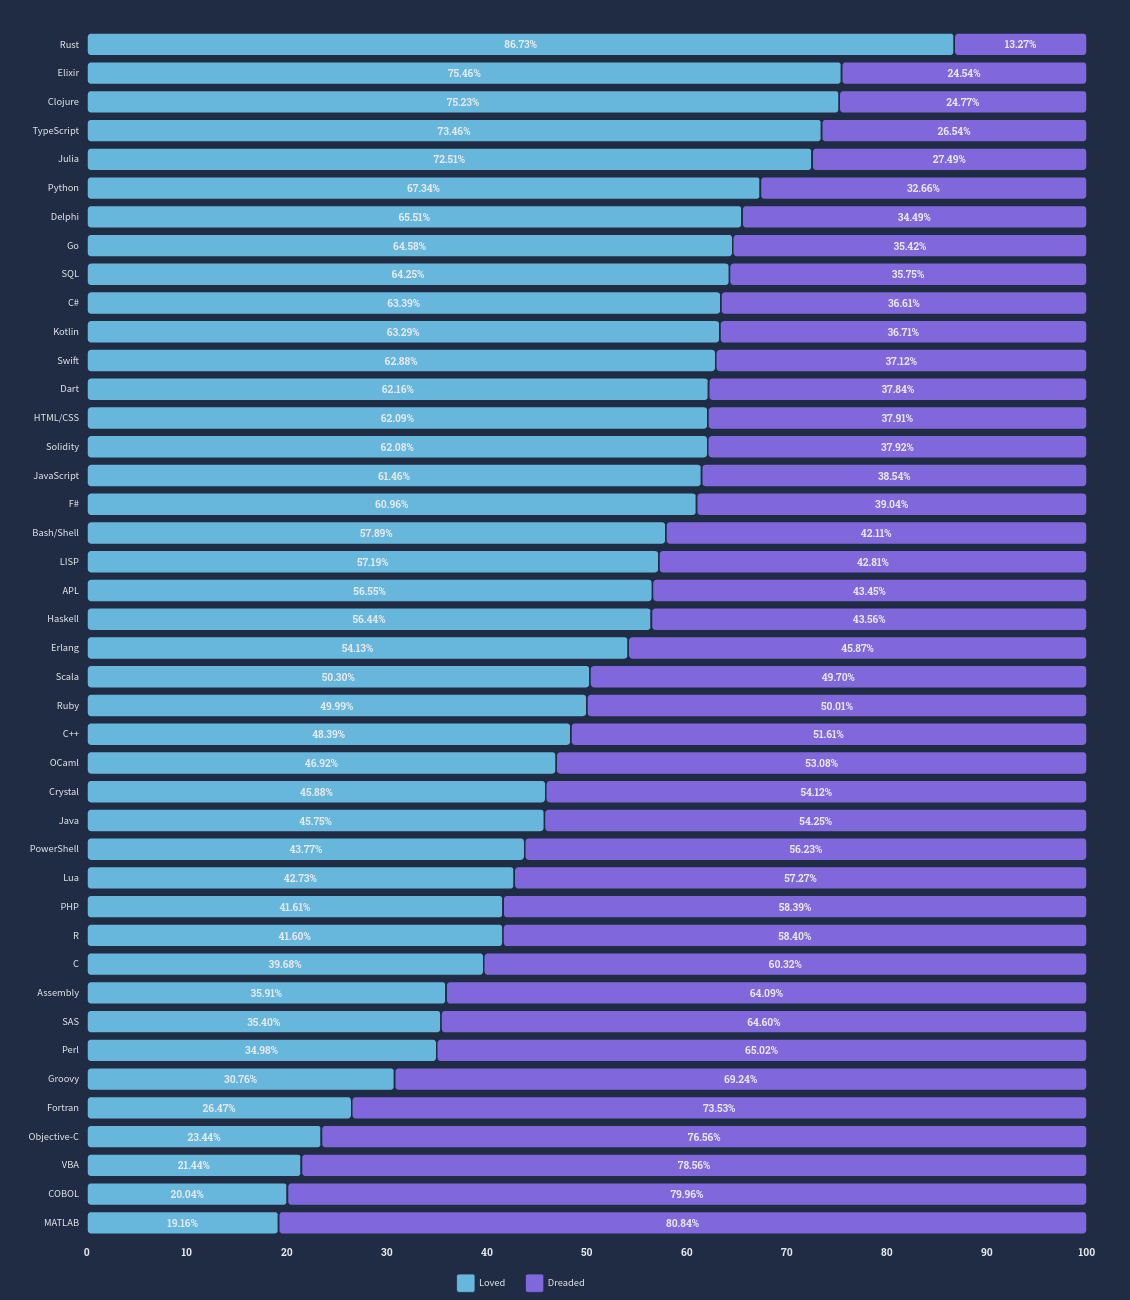
\includegraphics[width=\textwidth]{stack_loved}
  \caption{Wykres przedstawiający współczynnik uwielbiania/nienawiści danej technologii}
  \label{stack:loved}
  \caption*{Źródło: \url{https://survey.stackoverflow.co/2022}}
\end{figure}
\FloatBarrier

\subsection*{Yew}
Yew to framework umożliwiający tworzenie witryn WWW w języku Rust.
Z użyciem tej biblioteki możliwe jest konstruowanie niezawodnych
oraz wydajnych stron internetowych. Yew wykorzystuje WebAssembly wraz
z renderowaniem po stronie serwera, aby znacznie przyśpieszyć działanie
aplikacji na docelowej platformie. Umożliwia również na wykorzystanie 
funkcjonalności innych popularnych języków wykorzystywanych do tworzenia
aplikacji webowych takich jak JavaScript poprzez wykorzystanie biblioteki
wasm-bindgen udostępniającej standardową funkcjonalność tego języka oraz
pozwalającą na połączenie ze skryptami stworzonymi w tym języku.

Do tworzenia stron Yew wykorzystuje język podobny do HTML i JSX dzięki
czemu jest przystępny dla programistów mających wcześniejsze doświadczenie
z tymi technologiami. Podobnie jak inne środowiska takie jak React czy Angular
tworzone są komponenty, które mogą być wielokrotnie używane w różnych komponentach
oraz podstronach co sprawia, że kod jest czytelniejszy, zmniejszona jest jego złożoność
oraz możliwe jest wyeliminowanie niepotrzebnych powtórzeń.

\subsection*{Bootstrap}
Bootstrap to darmowe i otwarto-źródłowe środowisko programistyczne składające się
ze zbioru szablonów stworzonych w językach HTML, CSS i JavaScript, które mogą
być dowolnie wykorzystane z kompatybilnymi technologiami.
Ten framework zawiera podstawowe style potrzebne, aby stworzyć responsywną 
aplikacje webowe na wielu urządzeniach z różnymi rozmiarami ekranów oraz rozdzielczością. 

\subsection*{TypeScript}
TypeScript to darmowy, otwarto źródłowy stworzony oraz utrzymywane przez przedsiębiorstow Microsoft.
Jest rozszerzeniem popularnego języka JavaScript dodającym szeroko zastosowane funkcjonalności
w innych statycznie typowanych językach, tj. adnotacje typów oraz ich sprawdzanie
podczas kompilacji, interfejsy, typy wyliczeniowe czy uogólnienia.
Dodatkowo rozszerza język o słowa kluczowe async/await ułatwiające pracę
z asynchronicznymi funkcjami. Język TypeScript jest całkowicie kompatybilny ze 
środowiskami wspierającymi JavaScript - jest to język transpilowany do JS, a
dodatkowe funkcjonalności dostępne są jedynie podczas tworzenia oprogramowania.

Jego wykorzystanie w aplikacji zostało ograniczone jedynie do wykonania funkcjonalności,
których implementacja w pozostałych technologiach była niemożliwa lub znacznie 
utrudniona. Są to głównie funkcje pomocnicze wywoływane w odpowiednich komponentach
stworzonych w technologii Yew.

\section{Aplikacja serwerowa}

\subsection*{.NET Core}
.NET Core to następca popularnej platformy programistycznej .NET Framework stworzonej przez
firmę Microsoft. W przeciwieństwie do poprzednika, którego oficjalne wsparcie ograniczone było
do systemu Windows, a same oprogramowanie było własnościowe, jest to technologia otwarto-źródłowa
wspierająca wiele systemów operacyjnych \cite{price2021c}. Możliwe jest to poprzez zastosowanie
języka pośredniego niezależnego od systemu lub sprzętu. Instrukcje te tłumaczone są w 
wirtualnej maszynie CLR (ang. \textit{Common Language Runtime}) na język maszynowy, a
następnie wykonywane jak standardowy natywny kod \cite{msdn:clr}. Dzięki takiemu podjeściu
możliwe jest wytworzenie przenośnego oprogramowania, które może być wykorzystane na wielu
systemach.

\subsection*{C\#}
C\# to silnie typowany język obiektowy wysokiego poziomu stworzony przez firmę Microsoft.
Do kompilacji wykorzystywane jest środowisko .NET, dzięki czemu zachowane są
jego cechy takie jak przenośność oprogramowania oraz możliwość wykorzystania
innych języków programowania bazujących na tej technologii.

Dzięki automatycznemu zarządzaniu pamięcią ułatwia znacznie tworzenie
oprogramowania, gdyż w bezpiecznym kontekście nie pozwala na 
błędne jej wykorzystanie. Wykonywane jest to poprzez zastosowanie
mechanizmu odśmiecania pamięci (ang. \textit{garbage collection}).

C\# zawiera również rozszerzenia kolekcji LINQ (ang. \textit{Language Integrated Query})
pozwalające na wykonywanie na nich dodatkowych operacji, tj. grupowanie, sortowanie czy wyszukiwanie.
Te dodatkowe metody mogą być wykorzystane do działań na róznych źródłach danych takich jak dokumenty XML
czy też bazy danych SQL \cite{zhang2014}. Ich wysokopoziomowy kod jest przenośny i może być
wykorzystywany w takiej samej formie przy różnych źródłach danych.

Kolejną zaletą tej technologii jest możliwość wykorzystania meta-programowania. 
Jest to technika umożliwiająca modyfikację kodu podczas jego kompilacji lub wykonywania. 
Dzięki niej podczas wykonywania programu, poprzez refleksję, możliwe jest rozpoznanie
typu obiektu oraz jego modyfikacja. Pozwala również na tworzenie drzew wyrażeń, które
mogą zostać dynamicznie skompilowane w celu, np. wykorzystania zaawansowanej logiki
biznesowej, która może być zmienna.

\subsection*{ASP.NET}
ASP.NET to modularna platforma programistyczna oparta na technologii .NET. 
Jej bogata funkcjonalność pozwala na tworzenie stron internetowych, API HTTP oraz 
wiele innych aplikacji webowych poprzez zastosowanie wielu z jej rozszerzeń.
Jednym z nich jest wstrzykiwanie zależności (ang. \textit{dependency injection})
pozwalające na uzyskanie rozwiązania podobnego do wzorca architektury inwersji
kontroli (ang. \textit{Inversion of Control}). W takiej architekturze, zamiast
polegać na szczegółowej implementacji danej funkcjonalności czy serwisu,
użytkownik otrzymuje interfejs mówiący jedynie o tym do czego jest on przeznaczony.
Dzięki temu uzyskany kod jest całkowicie oddzielny od implementacji i pozwala
na znaczne ograniczenie efektów ubocznych przy działaniach takich jak refaktoryzacja,
restrukturyzacja czy przenoszenie implementacji, aby ta korzystały z innej biblioteki, np.
przy zmianie systemu bazodanowego.

Poprzez zastosowanie tak zwanych pośredników (ang. \textit{Middleware}) ASP.NET udostępnia
bardzo modularną oraz modyfikowalną strukturę przetwarzania zapytań HTTP.
Są to proste kroki, w których wykonywana jest logika związana z zapytaniem lub odpowiedzią
wysyłaną przez serwer. Podczas ich wykonania możliwy jest dostęp do danych zawartych
w zapytania oraz następnie jego modyfikacja, jak również decyzja o tym czy powinno
być ono propagowane do dalszych warstw. Przydatne to jest w przypadku, np. autoryzacji
gdzie w module sprawdzającym tożsamość użytkownika możliwe jest modyfikacja oraz zwrócenie
odpowiedzi o nieautoryzowanym dostępie i nie przekazywanie zapytania dalej do warstw, które zajmują
się dostępem do danych. Możliwe jest również zastosowanie innych pośredników takich
jak przechowywanie zapytań oraz odpowiedzi na nie w pamięci podręcznej, co znacznie
zwiększa wydajność systemu przy wielu takich samych zapytaniach. Poza wieloma wbudowanymi
pośrednikami programista sam może definiować swoją własną logikę oraz umieszczać
ją w odpowiednim momencie łańcucha wykonania.

\subsection*{MongoDB}
MongoDB to wieloplatformowy system bazodanowy. Dane przechowywane są w postaci dokumentów,
w formacie podobnym do JSON (ang. \textit{JavaScript Object Notation}), określaną nazwą
BSON (ang. \textit{Binary JSON}). Główną różnicą między tymi formatami jest sposób kodowania
danych - w przypadku formatu JSON jest to postać znaków UTF-8, a BSON jest to zapis binarny.
Pozwala to na łatwą konwersję między tymi typami, czyli co za tym idzie również uzyskiwanie
czytelnych dla człowieka danych, tym samym oszczędzając miejsce potrzebne do przechowywania
informacji jak również przyśpieszenie niektórych operacji jak indeksowanie.

W porównaniu do klasycznych baz danych SQL, MongoDB pozwala na większą elastyczność dzięki braku
konieczności określania schematu tabel. Wszystkie schematy są dynamiczne i mogą w dowolnym momencie 
zostać zmienione w celu dodania dodatkowych informacji jednocześnie nie zmieniając pozostałych
danych zapisanych w danej kolekcji. Jednocześnie ten system pozwala na tworzenie 
walidatorów kolekcji, co przydaje się w momentach kiedy chcemy uzyskać większą kontrolę
nad strukturą danych.

\subsection*{Docker}
Docker to zbiór oprogramowania umożliwiający dystrybucję oprogramowania jako tzw. kontener.
Są to wyspecjalizowane maszyny wirtualne, zawierające jedynie oprogramowanie potrzebne
do uruchomienia danego rozwiązania. Podobnie jak zwykłe rozwiązania wirtualizacyjne
są one od siebie odizolowane, ale w przeciwieństwie do innych, klasycznych rozwiązań
działają one na tym samym jądrze systemu operacyjnego dzięki czemu zużywają znacznie
mniej zasobów\cite{docker:what_is_container}. Odpowiednio skonfigurowane połączenia
między maszynami umożliwiają komunikację, np. poprzez protokół TCP. 
Po odpowiednim spakowaniu obrazu ta technologia umożliwia wykorzystanie identycznego
oprogramowania w różnych środowiskach niezależnie od systemu operacyjnego hosta.

Oprogramowaniem, które wchodzi w skład tego kompleksu i zostało ekstensywnie wykorzystane 
w realizacji projektu jest docker-compose. Te narzędzie wykorzystuje pliki konfiguracyjne
w formacie YAML, aby ułatwić pracę w środowiskach wymagających użycia kliku kontenerów, np.
w przypadku aplikacji serwerowej, która ma komunikować się z bazą danych.

\section{Urządzenie pomiarowe}
Urządzenie pomiarowe wykonane zostało na płytce Raspberry Pi Pico W, do którego z wykorzystaniem
portów ogólnego przeznaczenia GPIO podłączono sensory badające parametry środowiska.

\subsection*{Raspberry Pi Pico W}
Raspberry Pi Pico W to komputer jedno-płytkowy zbudowany na podstawie mikrokontrolera RP2040. 
Do głównych jego cech, które zostały wykorzystane do stworzenia systemu należą \cite{rp2040:datasheet}:
\begin{itemize}
  \item procesor dwurdzeniowy ARM Cortex-M0+,
  \item 264kB pamięci SRAM,
  \item 2MB pamięci flash,
  \item kontroller DMA (ang. \textit{Direct memory access}),
  \item 30 pinów GPIO (ang. \textit{General-purpose input/output}),
  \item 2 kontrollery SPI (ang. \textit{Direct memory access}),
  \item 2 kontrollery I2C (ang. \textit{Serial Peripheral Interface}),
  \item 16 kanałów PWM (ang. \textit{Pulse-width modulation}).
\end{itemize}
Płytka umożliwia łączność z siecią Wi-Fi przy użyciu wbudowanego chipu CYW43439
obsługujący standard 802.11n, który w odpowiednich warunkach pozwala na łączność
z prędkością do 600Mb/s. Wraz z nowszymi wersjami SDK umożliwia również wykorzystanie
całego potencjału tego urządzenia i umożliwia na połączenia protokołem Bluetooth.

Aktualnie dostępne oprogramowanie pozwala tworzyć systemy w językach programowania takich jak
Assembly, C, C++, Python oraz Rust. Istnieje również nieoficjalne wsparcie dla środowiska
Arduino oraz możliwość wykorzystania istniejących na tą platformę bibliotek.
Ze względu na język, w którym utworzono SDK (ang. \textit{Software Development Kit}) dla
tej platformy (język programowania C), najczęściej wykorzystywane są języki C oraz C++
ze względu na wysoki stopień kompatybilności.

\subsection*{C++}
C++ to obiektowy język programowania wysokiego poziomu, będący często określany jako
rozszerzenie języka C często używanego do tworzenia oprogramowania na systemy wbudowane.
Obsługuje on wysokopoziomowe abstrakcje takie jak obiekty, programowanie generyczne czy
abstrakcje pozwalając w tym samym czasie na używanie niskopoziomowej funkcjonalności 
takiej jak zarządzenie pamięcią czy dostęp do rejestrów procesora oraz używanie języka asembler.
Przez te cechy używany jest tam, gdzie potrzebna jest wysoka wydajność lub zasoby komputerowe
są znacznie ograniczone, np. serwery WWW, gry komputerowe czy systemy wbudowane.

W porównaniu do C zawiera również rozbudowaną standardową bibliotekę klas i funkcji.
Dodaje ona dodatkową funkcjonalność taką jak zaawansowane typy pozwalające na
przechowywanie zmiennej liczby danych, algorytmy takie jak sortowanie czy 
generowanie liczb losowych, obsługa plików, czasu oraz wielowątkowości.


\nocite{*} %wszystkie wpisy w bibliografi
\Urlmuskip=0mu plus 1mu\relax
\def\UrlBreaks{\do\/\do-}
\bibliographystyle{plain} %{latex8} posortowane wzgledem wystepowania
\bibliography{bibliografia}%

%\biblioteka{tak} % tak/nie
\end{document}
